\section{Evaluation protocol}
\label{sec:protocol}

\begin{figure}[htbp]
\centering
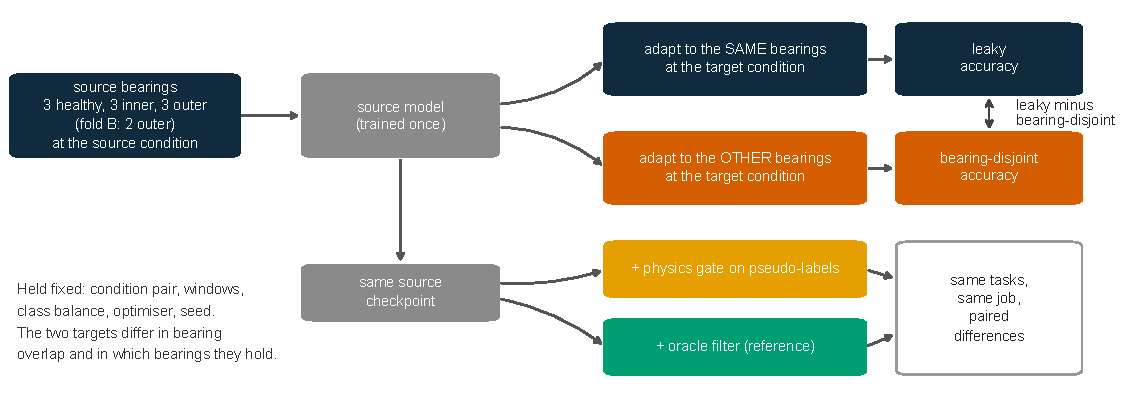
\includegraphics[width=\linewidth]{figures/fig1_design.pdf}
\caption{The paired design. One source model is trained on the source bearings at the source condition and then adapted
twice: to the \emph{same} bearings at the target condition (leaky) and to the complementary bearings at the same target
condition (bearing-disjoint, or clean). Both targets share the operating condition, the window contract and the class
balance. Gated and oracle arms reuse the same source checkpoint inside the same job, so their comparison with the ungated
clean arm is paired.}
\label{fig:design}
\end{figure}

\subsection{The paired leaky/clean design}

A source bearing set of 3 healthy, 3 outer-race and 3 inner-race specimens is trained at one operating condition. The
resulting source model is then adapted, without target labels, to two different targets at the same target condition
(Fig.~\ref{fig:design}): the \emph{leaky} target, made of the same physical bearings, and the \emph{clean} target, made of
the complementary bearings. Operating condition, window length, number of windows per class, class balance, optimiser,
schedule and seed are held fixed, as in the fixed-training designs of Vieira et al.\ \cite{vieira2026}. The leaky--clean
difference, written $\Delta_{\mathrm{leak}}$, therefore measures bearing overlap \emph{together with} the difference between
the two bearing sets, which hold different specimens. Two further contrasts separate these. The \emph{source-only}
difference is the same contrast for the source model before any adaptation step, read from the batch-0 accuracy that
every adaptation log records; it shows whether adaptation creates, amplifies or repairs the gap. The \emph{within-bearing}
contrast uses the ten random splits, in which every bearing is in the source in some splits and in the clean target in
others: for each bearing, its accuracy when seen minus its accuracy when unseen holds the specimen fixed. With three
conditions there are six ordered condition pairs, hence six tasks per split and per direction.

Windows are 2048 samples with 2000 windows per class; no window crosses a recording boundary. Within each recording the
windows start at evenly spaced positions and do not overlap: 33 or 34 windows per recording of about 256\,800 samples, a
hop of about 7\,700--7\,900 samples. The window length and the count per class are those of SDALR \cite{sdalr2025}, which
states neither a hop nor start positions; its preprocessed archive was not used, so the hop is our choice. Balance is per
class, not per bearing: a class with three bearings holds 680, 660 and 660 windows. Fold~B has only two real outer-race
bearings (KA22, KA30), so its outer-race class holds 1000 windows from each, 50 per recording. Because every target holds the same number of
windows per class, window accuracy equals balanced accuracy (the mean of the per-class recalls), so a three-class model
that ignores its input scores \SI{33.3}{\percent}.

\subsection{Splits}

\begin{table}[htbp]
\centering
\caption{Source bearing sets on Paderborn. The two mechanical folds are not symmetric: fold~B has two outer-race source bearings (KA22, KA30), not three, because the real-damage pool holds five.}
\label{tab:splits}
\small
\setlength{\tabcolsep}{4pt}
\begin{tabular}{llll}
\toprule
Split & Healthy & Outer race & Inner race \\
\midrule
fold A & K001, K002, K003 & KA04, KA15, KA16 & KI04, KI14, KI16 \\
fold B & K004, K005, K006 & KA22, KA30 & KI17, KI18, KI21 \\
\midrule
S00 & K001, K003, K004 & KA16, KA22, KA30 & KI04, KI16, KI18 \\
S01 & K002, K004, K006 & KA15, KA22, KA30 & KI04, KI17, KI21 \\
S02 & K002, K003, K005 & KA15, KA16, KA30 & KI16, KI17, KI21 \\
S03 & K002, K003, K004 & KA04, KA16, KA22 & KI16, KI18, KI21 \\
S04 & K001, K002, K006 & KA15, KA16, KA30 & KI04, KI14, KI18 \\
S05 & K003, K005, K006 & KA04, KA16, KA30 & KI04, KI17, KI21 \\
S06 & K002, K003, K006 & KA16, KA22, KA30 & KI04, KI17, KI18 \\
S07 & K003, K005, K006 & KA04, KA16, KA22 & KI04, KI14, KI16 \\
S08 & K001, K002, K006 & KA15, KA22, KA30 & KI04, KI16, KI21 \\
S09 & K002, K003, K005 & KA04, KA15, KA16 & KI16, KI17, KI21 \\
\bottomrule
\end{tabular}
\begin{minipage}{\linewidth}\vspace{2pt}\footnotesize The clean target of each row is the complement within the real-damage pool (6 healthy, 5 outer-race, 6 inner-race); the leaky target is the same bearings at the target operating condition. S00--S09 were drawn uniformly without replacement from the 4{,}000 possible 3/3/3 draws with a seed fixed before any run.\end{minipage}
\end{table}


Two families of splits are used on Paderborn (Table~\ref{tab:splits}). The two \emph{mechanical folds} follow a fixed rule
--- within each (damage origin, fault type) group, sort bearing codes lexicographically and assign the first half to fold A
--- and are run in both directions, which gives 12 paired tasks. Because two folds are two draws out of the 4000 possible
3/3/3 source sets, we drew ten source sets uniformly without replacement from those 4000, excluding fold A, with the seed
and the draw list committed before any of these runs. The \emph{split} is the statistical unit for the ten-split analyses;
tasks are the unit within a fold. On HUST the same construction uses bearing types: the source is three of the five types
and the clean target the other two, for six pre-registered splits.

\subsection{Adaptation variants}

SDALR is run from its released code with two checkpoint policies. \texttt{as\_released} keeps the released selection rule,
which compares target accuracy against its initial value and therefore consults target labels; \texttt{final\_checkpoint}
takes the last iterate and touches no target label. All headline numbers use \texttt{final\_checkpoint};
\texttt{as\_released} is reported once, in Section~\ref{sec:res-collapse}. SHOT is our implementation of the published
template on the same backbone, data pipeline, schedule and source checkpoint, with a frozen classifier head, the
information-maximisation loss and centroid pseudo-labels recomputed each epoch, evaluated at the last iterate.

\subsection{Gating and the oracle reference}

A gate returns one verdict per \emph{recording}, in $\{\text{silent},\text{inner race},\text{outer race}\}$, which every
window of that recording inherits; silence is not a healthy verdict. Inside the adaptation loop the verdict acts on SDALR's
pseudo-label step: where the gate speaks, a pseudo-label is kept only if it agrees with the verdict and is otherwise
withheld from the supervised term (the window still enters SDALR's entropy term, as SDALR's own unreliable samples do);
where the gate is silent, the method is unchanged. The \emph{oracle filter} replaces the verdict by the true label of each
window, keeping only correct pseudo-labels. It is a reference, not a proven bound: adaptation is non-convex, and a filter
that also withheld some correct labels could in principle do better. Like every arm, it is scored on the target windows it
adapts on, as is standard in SFDA.

All arms of a comparison --- ungated, each gate, oracle --- run in one job from the same source checkpoint with the same
seed; we verify this from identical batch-0 accuracy in every adaptation log. Write $a_{\mathrm{leaky}}$,
$a_{\mathrm{clean}}$ and $a_{\mathrm{oracle}}$ for the ungated leaky, ungated clean and oracle-filtered clean accuracy, each
the mean over the six condition pairs of a split. The collapse is split as
\begin{equation}
\underbrace{a_{\mathrm{leaky}}-a_{\mathrm{clean}}}_{\text{total}}
=\underbrace{\left(a_{\mathrm{oracle}}-a_{\mathrm{clean}}\right)}_{\text{recovered by the oracle filter}}
+\underbrace{\left(a_{\mathrm{leaky}}-a_{\mathrm{oracle}}\right)}_{\text{not recovered}}.
\label{eq:decomp}
\end{equation}
The second term mixes what the source model carries with the difference in difficulty between the two bearing sets, and
can be negative.

\subsection{Statistics}

Effects are paired differences. Within a fold the twelve tasks share source checkpoints, so task-level tests are
pseudo-replicated; every primary effect is therefore tested with the source fold or the split as the cluster, by an exact
permutation test that flips the sign of whole clusters, and summarised by its median with a percentile bootstrap interval
over clusters (20\,000 resamples). With two folds a cluster-level test cannot fall below $p = 0.25$, so \emph{the fold
experiments are descriptive and the ten random splits carry the inference}. The splits share bearings --- a pool of 17
cannot supply ten disjoint source sets --- so sign-flip exchangeability holds only approximately, and the inference is
conditional on this pool of bearings; the within-bearing contrast is reported beside it for that reason. Cluster-level
$p$-values of the ten primary tests fixed before revision six --- the collapse on the folds and on the ten splits, the
envelope and comb gate gains on the folds and the envelope gain on the splits, the two random-forest collapses and the
same-condition control on the splits, the SHOT collapse on the splits and the HUST collapse on its six splits --- are
adjusted together by Benjamini--Hochberg \cite{benjamini1995}, which holds under positive dependence \cite{benjamini2001}, and
by Benjamini--Yekutieli, which holds under any dependence. Every ten-split result survives both (largest
$p_{\mathrm{BY}} = 0.014$); HUST survives the first but not the second ($p_{\mathrm{BY}} = 0.065$), because six clusters
cannot produce a raw $p$ below 0.016, and is described as replicating direction and size. Analyses added in this
revision (source-only arm, within-bearing contrast, spillover, purity, intervals) are post-hoc and descriptive; the two new
experiments (source-diversity curve, kinematic-feature forest) were pre-registered with decision rules before they ran.
False-acceptance counts carry intervals from a bootstrap over the six healthy bearings or, for counts of zero or one, exact
Clopper--Pearson intervals over records.

\subsection{Reproducibility, jobs and pre-specification}

Every effect here is a difference between two runs, so we measured the difference produced by no change at all: every
retained re-execution of the gating configuration --- eleven arm pairs over 66 paired tasks on both folds --- reproduces the
first execution to the last reported decimal. The pipeline is deterministic under a fixed seed and code path, and the
relevant null for a single comparison is the random trajectory itself, whose between-seed range for the ungated clean fold
mean is 3.2 points on fold~A and 1.9 on fold~B.

The fold experiments ran in two jobs at two code revisions: a fold job, which produced the leaky and clean arms, and a later
gating job, which produced the ungated, gated and oracle clean arms. The later revision wraps SDALR's evaluation routine to
save per-window predictions; source pretraining calls that routine on its validation loader halfway through training, and
creating the extra loader iterator advances the global random generator. From that point the source pretraining follows a
different trajectory, and the two jobs train different source checkpoints: their batch-0 target accuracy differs by up to
9.3 points on fold~A and 2.5 on fold~B, and their ungated clean fold-A means are \SI{58.4}{} and \SI{56.8}{\percent}. Arms are
therefore never compared across jobs. Leaky--clean contrasts come from the fold job, gated and oracle arms are compared with
the gating job's own ungated arm, and the fold-level oracle decomposition, which would need a leaky arm the gating job never
ran, is not reported. All ten random splits ran every arm in one job.

Every hypothesis, decision rule, arm and budget was written into a version-controlled protocol before the corresponding
run, including the gate operating points ($z = 10$ for the envelope rule, $\alpha = 0.05$ for the comb tests). The protocol
is a file in the project repository rather than a registry entry, so we call it pre-specification; each entry carries the
commit that introduced it, every result artifact the commit that produced it, and the repository with its history is
archived with the submission. Results that failed their rule are reported as such, one planned remedy experiment was cut
for budget before any of its outcomes were seen, and every reported number carries a run identifier in an append-only ledger
with the retained artifact and its checksum (Supplementary~S4).

\paragraph{AI-assisted execution.} An AI coding assistant (Claude, Anthropic, used through the Claude Code agent; this
revision used the model \texttt{claude-opus-5-5}) wrote and ran analysis, evaluation and figure code, prepared and
submitted compute jobs, and cross-checked numbers against the retained artifacts. Hypotheses, decision rules and operating
points were fixed in the protocol by the author before the corresponding runs. Every result traces to a retained artifact
produced by a recorded job, and the code is released, so each step is reproducible without the assistant. The author
verified the analyses by re-running the analysis scripts against the artifacts and takes full responsibility for the content.
